\begin{frame}
  \titlepage
\end{frame}

\begin{frame}{A useful integration asks a precise question}
  \begin{itemize}
    \item Authenticate with the right account and key.
    \item Choose event or attribute scope.
    \item Set filters and export policy explicitly.
    \item Traverse pages without losing records.
    \item Handle updates, failures and removals deliberately.
  \end{itemize}
  \begin{block}{Reference snapshot}
    MISP 2.5.50, reviewed 29 October 2026. Check your deployed version.
  \end{block}
  \note{Allow 40--50 minutes for the presentation and another 30--40 for the
  workshop. Learners need basic HTTP and JSON knowledge. This replaces a lesson
  about the original API redesign with current operational contracts.
  The README pins MISP and PyMISP source revisions; patch levels, permissions,
  settings and exporters affect behaviour.}
\end{frame}

\section{Make one request}

\begin{frame}{The API uses your account's visibility}
  \centering
  \begin{tikzpicture}[
    node distance=.40cm,
    stage/.style={draw=mispTeal,rounded corners,fill=mispBlue!5,
      text width=8.1cm,align=center,minimum height=.65cm,font=\small},
    flow/.style={-{Stealth},thick,draw=mispTeal}]
    \node[stage] (key) {Authenticate account and key};
    \node[stage,below=of key] (scope) {Apply role, data visibility and query filters};
    \node[stage,below=of scope] (format) {Export in the requested scope and format};
    \node[stage,below=of format] (client) {Validate, interpret and store the result};
    \draw[flow] (key)--(scope);
    \draw[flow] (scope)--(format);
    \draw[flow] (format)--(client);
  \end{tikzpicture}
  \note{An API key is not a bypass around organisation, distribution or sharing
  group visibility. A site-admin test alone does not verify an analyst-facing
  integration. In the lab, an ordinary user in the owning org saw five synthetic
  domain attributes while a user in a different org saw only its own private
  fixture. API operation permission and data visibility are separate checks.}
\end{frame}

\begin{frame}{Set up a key for the task}
  \begin{itemize}
    \item The account needs API access: \code{perm_auth}.
    \item Send the raw key in \code{Authorization}.
    \item Advanced keys can restrict expiry, source IP and writes.
    \item Keep keys outside scripts, notebooks and shared collections.
  \end{itemize}
  \begin{alertblock}{Read-only does not mean GET-only}
    A read-only key can POST a search, while event creation is denied.
  \end{alertblock}
  \note{There is no Bearer prefix in the normal MISP Authorization header.
  AuthKey restrictions are combined with the user's role and data visibility.
  Generate and manage keys through the profile/auth-key UI under your instance's
  policy. Advanced keys are displayed once. The live test used an expiring
  read-only key for an ordinary User, successfully POSTed searches and received
  HTTP 403 when attempting event creation.}
\end{frame}

\begin{frame}[fragile]{First request: inspect the instance}
\begin{lstlisting}[language=bash]
curl --fail-with-body --silent --show-error \
  --connect-timeout 5 --max-time 60 \
  -H "Authorization: $MISP_API_KEY" \
  -H 'Accept: application/json' \
  "$MISP_URL/servers/getVersion"
\end{lstlisting}
  Read \code{version} and \code{pymisp_recommended_version}.

  Keep TLS verification enabled; supply your organisation's CA bundle if needed.
  \note{Set URL and key locally before the command; never paste a working key
  into the slides. MISP\_URL is the base URL including any deployment subdirectory
  and without a trailing slash for these curl examples. CURL\_CA\_BUNDLE and
  REQUESTS\_CA\_BUNDLE can supply private CA trust. Check 4xx, redirects, login HTML
  and server errors before trying a broad data export. The Python sample allows
  plaintext HTTP only for an isolated loopback lab.}
\end{frame}

\begin{frame}{Choose the endpoint by the result you need}
  \small
  \begin{tabular}{P{.45\textwidth}P{.45\textwidth}}
    \toprule
    Endpoint & Result \\
    \midrule
    \code{/events/index} & Event summaries \\
    \code{/events/restSearch} & Full events or metadata \\
    \code{/attributes/restSearch} & Matching attributes \\
    \code{/events/view/{uuid}} & One known event \\
    \bottomrule
  \end{tabular}
  \medskip
  Use POST with a JSON body for search. Read each endpoint's contract.
  \note{The first three endpoints support the POST search patterns taught here;
  event view is a GET. Current restSearch also supports objects, sightings and
  galaxy clusters, each with different parameters and formats. Do not claim
  every MISP endpoint uses one universal query or response schema. Deployment
  prefix handling matters when building URLs.}
\end{frame}

\begin{frame}[fragile]{A bounded attribute request}
\begin{lstlisting}[language=json]
{
  "returnFormat": "json",
  "type": "domain",
  "value": "%.example",
  "published": [0, 1],
  "to_ids": [0, 1],
  "includeEventTags": true,
  "limit": 100,
  "page": 1
}
\end{lstlisting}
  \code{POST /attributes/restSearch}
  \note{The complete file also requests event UUIDs and a stable ID order.
  Reserved .example names make the fixture recognisable. An empty result is
  correct before creating training data. These raw JSON flag arrays include
  both states deliberately. Set Accept and Content-Type to application/json.
  The example does not request attachments or broad enrichment data.}
\end{frame}

\begin{frame}[fragile]{The response envelope depends on the scope}
  \begin{block}{Attribute search}
\begin{lstlisting}[language=json]
{"response": {"Attribute": [
  {"uuid": "...", "type": "domain", "value": "..."}
]}}
\end{lstlisting}
  \end{block}
  \begin{block}{Event search}
\begin{lstlisting}[language=json]
{"response": [
  {"Event": {"uuid": "...", "info": "..."}}
]}
\end{lstlisting}
  \end{block}
  \note{The ellipses are structural illustrations, not runnable fixture UUIDs.
  Event index instead returns a flat summary array, and event view returns an
  Event object. Validate the expected envelope before consuming it.
  PyMISP removes the outer response wrapper and can construct typed objects,
  so raw HTTP parsers must not be reused on pythonified results.}
\end{frame}

\section{Search with intent}

\begin{frame}{A matching event can contain other attributes}
  \begin{block}{Event scope}
    Find an event through a domain match; full JSON can also include the
    event's IP address and contextual attributes.
  \end{block}
  \begin{block}{Attribute scope}
    Return the attributes that match the attribute query.
  \end{block}
  \medskip
  Use \code{metadata: true} for lighter event results.
  \note{The live fixture had domain and ip-dst attributes. An event search
  filtered by type domain still returned the contextual IP in its full JSON.
  This is useful for analysis but matters when constructing a detection feed.
  Metadata is a deliberate reduced representation, not a complete event with
  no attributes. Include the scope in downstream data contracts.}
\end{frame}

\begin{frame}{Exact values and wildcard values are different}
  \begin{center}
    \begin{tabular}{ll}
      \toprule
      Filter value & Intent \\
      \midrule
      \code{workshop.example} & Exact attribute value \\
      \texttt{\%.example} & Suffix match \\
      \texttt{\%REST API training\%} & Event-info substring \\
      \bottomrule
    \end{tabular}
  \end{center}
  \medskip
  Start with one known value or UUID. Add filters one at a time.
  \note{The event-info query initially returned zero when given only REST API
  training; the explicit wildcard form matched. The published example uses
  that tested form. These are supported SQL-style wildcard patterns, not a
  regex language. Exact/wildcard behaviour is field-specific; consult the
  deployed endpoint when extending the examples.}
\end{frame}

\begin{frame}{Select publication and detection flags explicitly}
  \small
  \begin{tabular}{P{.27\textwidth}P{.62\textwidth}}
    \toprule
    Raw JSON filter & Meaning \\
    \midrule
    \code{published: 1} & Published events \\
    \code{published: 0} & Unpublished events visible to the caller \\
    \code{to_ids: 1} & Detection-marked attributes \\
    \code{to_ids: 0} & Contextual attributes \\
    \code{[0, 1]} & Either state, for these raw JSON filters \\
    \bottomrule
  \end{tabular}
  \note{Use numeric 0 and 1 in these search examples. A literal false can skip
  the filter in the reviewed pipeline, so it is not universally equivalent to
  requesting zero. Create/edit payloads have their own boolean handling.
  PyMISP 2.5.34.4 rejects a to\_ids list despite the raw server accepting it.
  For its JSON non-restrictive search, omitting to\_ids includes both states.
  The raw live tests verified unpublished contextual attributes with numeric zeros.}
\end{frame}

\begin{frame}[fragile]{Express tag logic with explicit operators}
\begin{lstlisting}[language=json]
{
  "tags": {
    "AND": ["tlp:clear"],
    "OR": ["training:reviewed", "training:verified"],
    "NOT": ["training:exclude"]
  }
}
\end{lstlisting}
  Require the AND tag, one OR tag, and no NOT tag.
  \note{This illustrative combination requires the custom training tags to
  exist and be attached; it is not the supplied fixture's default query.
  The live tests separately verified AND, OR and NOT selection using the
  event's tlp:clear tag. Do not copy dashboard-specific include/exclude
  substring syntax into a restSearch tags object. A query filter is not
  an access-control policy.}
\end{frame}

\begin{frame}{Tags may come from the event}
  \begin{itemize}
    \item Event and attribute tags can both influence a match.
    \item \code{includeEventTags} adds inherited event tags to the result.
    \item Inspect the \code{inherited} marker before interpreting attachment.
  \end{itemize}
  \begin{block}{Keep context when exporting}
    A tag-driven match does not mean that tag was attached directly to
    every returned attribute.
  \end{block}
  \note{The JSON exporter marks included EventTag-derived tags as inherited.
  The lab verified that event-level tlp:clear selected both domain attributes
  and appeared with the inherited marker. Event-scope matching and attribute
  result selection have different granularity. Event-tag changes also matter
  for incremental consumers: an attribute timestamp alone need not describe
  every parent-context change.}
\end{frame}

\begin{frame}{Pick the clock that answers your question}
  \small
  \begin{tabular}{P{.40\textwidth}P{.50\textwidth}}
    \toprule
    Field & Clock \\
    \midrule
    \code{timestamp} & Change time in the selected scope \\
    \code{event_timestamp} & Parent event change time \\
    \code{publish_timestamp}, \code{last} & Event publication time \\
    \code{from}, \code{to} & Event date bounds \\
    \code{first_seen}, \code{last_seen} & Observation time \\
    \bottomrule
  \end{tabular}
  \note{For attributes, timestamp and the explicit attribute\_timestamp refer
  to attribute change time. Event timestamp is a separate field. Relative
  publication windows do not substitute for an update cursor, and observation
  time is not ingestion time. The range helper accepts inclusive lower and
  upper bounds. Use fixed Unix timestamps across a paginated run instead of
  recalculating a relative window on each page.}
\end{frame}

\begin{frame}{Changing the format can change the selection}
  \begin{columns}[T,onlytextwidth]
    \begin{column}{.47\textwidth}
      \begin{block}{JSON / CSV}
        Non-restrictive exporters in this snapshot.
        State selection explicitly when comparing results.
      \end{block}
    \end{column}
    \begin{column}{.49\textwidth}
      \begin{block}{Detection text}
        Defaults to published events and detection-marked attributes
        when those filters are omitted.
      \end{block}
    \end{column}
  \end{columns}
  \medskip
  An analysis result is not automatically a deployment policy.
  \note{MispAttribute::restSearch injects published=1 and to\_ids=1 when the
  exporter is restrictive. JsonExport and CsvExport declare themselves
  non-restrictive. TextExport does not. Defaults may vary by format and
  source revision. Explicit filters, warninglists, decay and handling
  restrictions deserve review before feeding a defensive system.}
\end{frame}

\begin{frame}[fragile]{A detection-policy exercise}
\begin{lstlisting}[language=json]
{
  "returnFormat": "text",
  "type": "domain", "value": "%.example",
  "published": 1, "to_ids": 1,
  "tags": {"AND": ["tlp:clear"],
           "NOT": ["training:exclude"]},
  "enforceWarninglist": true,
  "limit": 100, "page": 1
}
\end{lstlisting}
  Output is text. The unpublished workshop event correctly contributes nothing.
  \note{The file under examples contains the full request. The published lab
  fixture had a detection-marked domain and a contextual domain; only the
  detection-marked one appeared in this text export. The .example restriction
  keeps the exercise synthetic. Never deploy these fixture values as a real
  blocklist. Other formats such as STIX and IDS rules have their own
  compatibility and representation contracts.}
\end{frame}

\begin{frame}{Warninglist annotations and filtering differ}
  \begin{block}{Annotate}
    \code{includeWarninglistHits} adds matching-list information to JSON.
  \end{block}
  \begin{block}{Filter}
    \code{enforceWarninglist} can remove rows after query pagination.
  \end{block}
  \medskip
  Empty formatted output is not always proof that later pages have no candidates.
  \note{fetchAttributes applies warninglist enforcement after fetching rows
  and can skip them. A short or empty output page may therefore be misleading
  as a completion signal. The supplied pagination sample rejects post-query
  filter options and non-JSON formats rather than claiming one loop safely
  traverses every exporter. For those formats, inspect the deployed exporter
  and its count/skipped semantics and design a dedicated traversal.}
\end{frame}

\section{Automate and verify}

\begin{frame}{A role cap can make every page short}
  \begin{center}
    \begin{tabular}{lrl}
      \toprule
      Requested & Returned & Continue? \\
      \midrule
      Page 1, limit 100 & 2 & Yes \\
      Page 2, limit 100 & 2 & Yes \\
      Page 3, limit 100 & 1 & Yes \\
      Page 4, limit 100 & 0 & Stop for this plain JSON query \\
      \bottomrule
    \end{tabular}
  \end{center}
  \medskip
  Five records were available. Stopping at the first short page loses three.
  \note{This is the actual tested role-cap fixture: the ordinary User role had
  restsearch\_limit\_result set to two in the disposable lab. The event cap uses
  a scope-specific divisor, so it differed from the attribute cap.
  Do not request a higher-privilege key just to avoid pagination. The loop's
  empty-page rule is intentionally limited to the sample's supported JSON
  filters; it is not a universal export rule.}
\end{frame}

\begin{frame}{Bound the traversal and reject incomplete results}
  \begin{itemize}
    \item Start at page 1; request a deterministic order.
    \item Validate the envelope and attribute UUIDs.
    \item Continue through short pages.
    \item Fail on repeated UUIDs or a maximum-page bound.
    \item Publish output and checkpoints only after success.
  \end{itemize}
  \note{The example forces Attribute.id ASC and permits 1--1000 for page size
  and maximum pages, with defaults 100 and 20. A repeated UUID can indicate a
  repeated page or concurrent drift; it is treated as incomplete, not silently
  skipped. Stable sort does not create a database snapshot and does not solve
  every concurrent deletion or visibility change. X-Result-Count on restSearch
  is this render's count, not a universal global total or cursor.}
\end{frame}

\begin{frame}[fragile]{Use the supplied read-only Python client}
\begin{lstlisting}[language=bash]
python examples/search_attributes.py \
  --page-size 100 --max-pages 20 \
  > attributes.ndjson.tmp \
  && mv attributes.ndjson.tmp attributes.ndjson
\end{lstlisting}
  \begin{itemize}
    \item Environment-provided URL and key; trusted TLS.
    \item Timeouts, no redirects, JSON/envelope checks.
    \item A failure leaves partial output unpublished.
  \end{itemize}
  \note{Install the pinned requirements in a virtual environment first.
  The client's supported filter set is deliberately narrow and excludes
  attachment downloads and post-query warninglist/decay filtering. It does
  not save a checkpoint. Protect the temporary file as intelligence output.
  Requests keeps normal proxy and CA handling. Errors do not dump keys,
  headers or server response bodies. This is a teaching client, not a
  replacement for a production ingestion service or PyMISP.}
\end{frame}

\begin{frame}[fragile]{PyMISP offers a typed view of the same task}
\begin{lstlisting}[language=Python]
rows = misp.search(
    controller="attributes", return_format="json",
    type_attribute="domain", value="%.example",
    include_event_tags=True, include_event_uuid=True,
    limit=100, page=1, pythonify=True,
)
\end{lstlisting}
  Check for an error dictionary before treating the result as a list of objects.

  This is one page, not a complete export.
  \note{The companion constructs PyMISP with environment configuration, TLS
  verification and timeouts, and validates a list of MISPAttribute instances.
  Current client parameter names differ from raw JSON: type\_attribute rather
  than type, return\_format rather than returnFormat. Unknown kwargs are not
  a substitute for checking the server contract. Empty lists are valid.
  Do not use ExpandedPyMISP in the new lesson or assume list index zero exists.}
\end{frame}

\begin{frame}{Keep one fixed window for an incremental run}
  \begin{enumerate}
    \item Capture an upper timestamp at run start.
    \item Set the lower bound from the last successful run, with overlap.
    \item Fetch every page using the same inclusive bounds.
    \item Upsert by UUID and complete downstream writes.
    \item Advance the checkpoint only when the whole run succeeds.
  \end{enumerate}
  \note{A JSON timestamp range is [lower, upper], with inclusive comparisons.
  Choose a documented first-run backfill and overlap policy. Duplicate records
  across runs are expected with overlap and should be reconciled by UUID and
  version/change time. This is a design pattern, not an implemented guarantee
  in the supplied client. It does not capture every parent tag, distribution,
  access-loss or hard-deletion change; reconciliation remains necessary.}
\end{frame}

\begin{frame}{Plan for removals and lost visibility}
  \begin{itemize}
    \item Normal searches omit soft-deleted attributes.
    \item Tombstone visibility depends on permissions and endpoint.
    \item Hard deletion and lost access may provide no visible tombstone.
    \item Consumers need reconciliation, expiry and removal rules.
  \end{itemize}
  \begin{alertblock}{An empty deletion search proves very little}
    Check the caller's actual deletion-view contract.
  \end{alertblock}
  \note{In this source, attribute restSearch deleted=1 returned a tombstone to
  a sync-capable administrator but not the ordinary owning user. That owner
  could inspect the deleted record through events/view/UUID/deleted:1.
  fetchAttributes has a sync-permission condition for the numeric deleted
  option. Do not grant sync privileges just for the workshop or promise that
  any ordinary reader receives all removals. Use MISP server synchronisation
  for its intended purpose rather than replacing it with a naive polling loop.}
\end{frame}

\begin{frame}{Write a small, explicit change}
  \begin{center}
  \begin{tikzpicture}[
    node distance=.35cm,
    labstep/.style={draw=mispTeal,rounded corners,fill=mispBlue!5,
      text width=7.6cm,align=center,minimum height=.65cm,font=\small},
    flow/.style={-{Stealth},thick,draw=mispTeal}]
    \node[labstep] (create) {Create an unpublished, organisation-only event};
    \node[labstep,below=of create] (add) {Capture event UUID; add a synthetic attribute};
    \node[labstep,below=of add] (edit) {Capture attribute UUID; edit selected fields};
    \node[labstep,below=of edit] (verify) {Re-read, deliberately delete, verify and clean up};
    \draw[flow] (create)--(add);
    \draw[flow] (add)--(edit);
    \draw[flow] (edit)--(verify);
  \end{tikzpicture}
  \end{center}
  \note{The JSON files and README implement this sequence with no fixed IDs.
  The event omits date so the server supplies today's date. Distribution zero
  is organisation-only; the attribute inherits its event with distribution
  five. It is contextual and correlation-disabled for the exercise.
  Publishing is separate and can trigger sync or alerts; the learner's event
  stays unpublished. Do not run write exercises against production data.}
\end{frame}

\begin{frame}[fragile]{Update only the fields you intend}
\lstinputlisting[language=json]{examples/edit-attribute.json}
  \code{POST /attributes/edit/{attribute-uuid}}
  \medskip
  Re-read the attribute and verify the comment.
  \note{Do not replay the whole fetched event or attribute just to change one
  comment. It may include stale timestamps, distribution and unrelated data.
  Reconcile after a conflict. A timed-out write may have succeeded: blind
  retries can create duplicates or overwrite newer state. UUID identity helps
  reconcile operations, but is not universal idempotency for every endpoint.
  The lab verified this edit through an ordinary writer's own new attribute.}
\end{frame}

\begin{frame}{Use the built-in tools to inspect a request}
  \begin{columns}[c,onlytextwidth]
    \begin{column}{.58\textwidth}
      \centering
      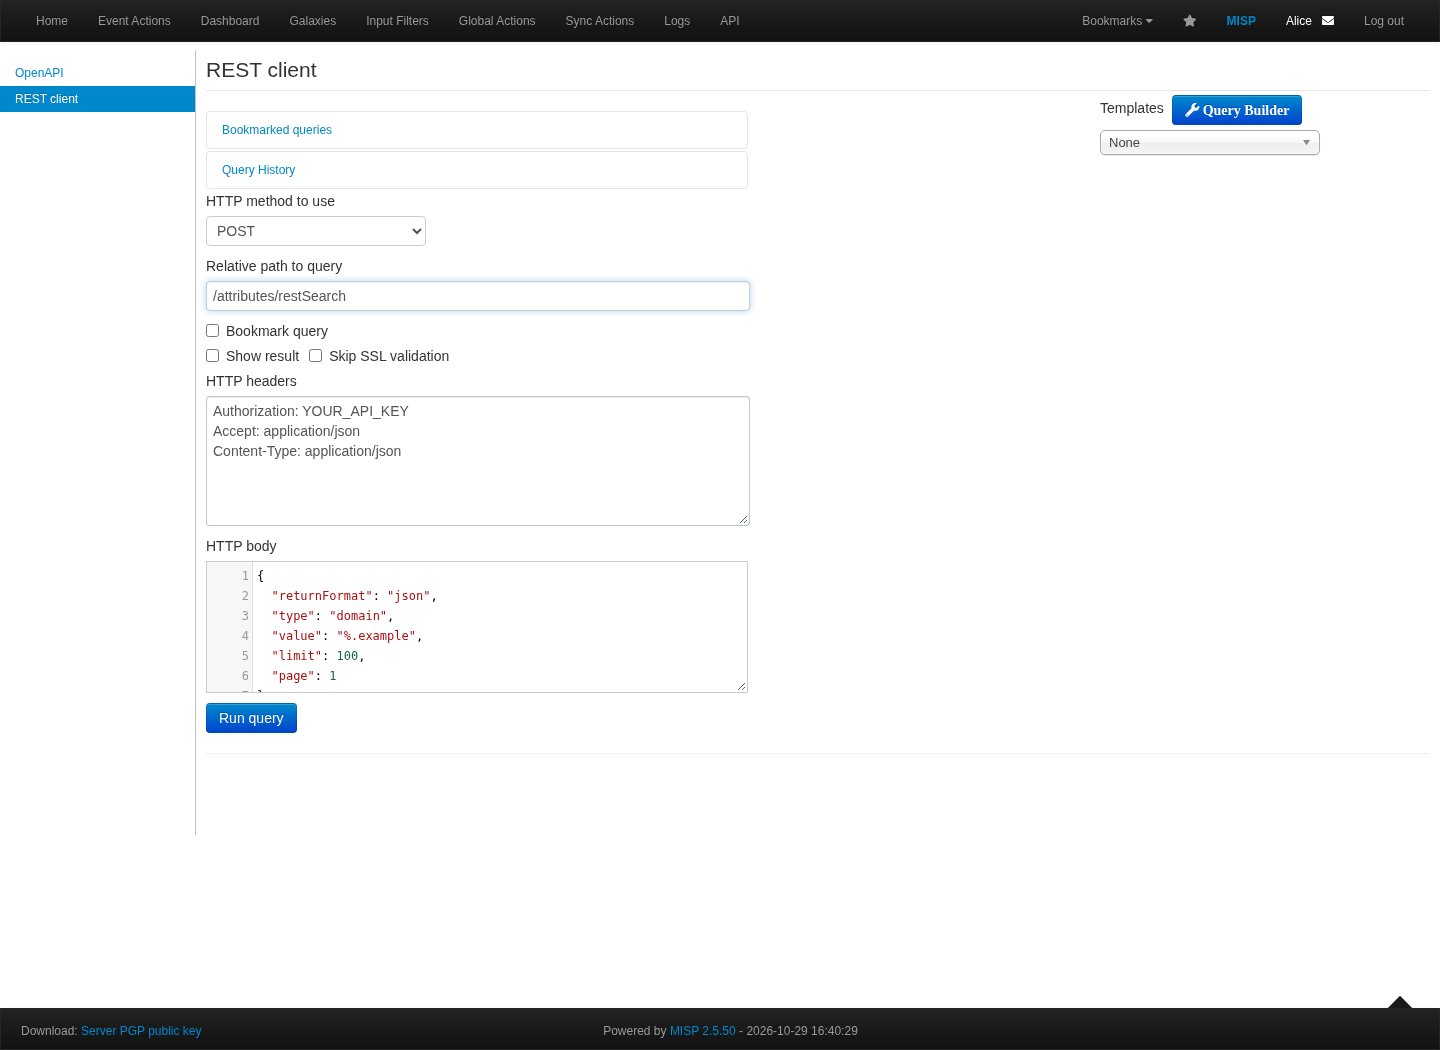
\includegraphics[width=\textwidth,height=5.8cm,keepaspectratio]{images/rest-client.png}
    \end{column}
    \begin{column}{.38\textwidth}
      \begin{itemize}
        \item \code{/api/rest}
        \item Templates and query builder.
        \item History and bookmarks.
        \item Generated request code.
      \end{itemize}
    \end{column}
  \end{columns}
  \note{This genuine 2.5.50 capture shows a prepared request with the visible
  YOUR\_API\_KEY placeholder and no submission. See the full-size README image
  for labels. The older servers/rest path redirects here. Review generated
  curl/Python before reuse: remove embedded keys, add timeouts and keep TLS
  verification. The deployed OpenAPI UI is at api/openapi.}
\end{frame}

\begin{frame}{Try the read-only notebook and Postman collection}
  \begin{block}{Notebook}
    Raw page, bounded traversal and typed PyMISP page. No saved keys or outputs.
  \end{block}
  \begin{block}{Postman}
    Version, attribute JSON, event metadata, policy text and CSV:
    five requests, ten assertions.
  \end{block}
  \medskip
  Keep the filled Postman environment and notebook results local.
  \note{The committed environment has a blank secret api\_key and a placeholder
  base URL. The actual collection was executed with Newman against the lab's
  read-only key. It checks the response status and relevant envelope/type;
  each request is a single page. The notebook cells never create or delete
  records. Mutation is deliberate through the separate workshop instructions.
  Older notebooks, collections and executable samples live only in the archive.}
\end{frame}

\begin{frame}{Classify failure before retrying}
  \small
  \begin{tabular}{P{.25\textwidth}P{.65\textwidth}}
    \toprule
    Symptom & Next check \\
    \midrule
    401 / 403 & Key, expiry, IP, role and endpoint permissions \\
    404 & Base path, UUID, existence and caller visibility \\
    400 / 405 & Method, JSON shape, types and validation \\
    HTML / redirect & Login or proxy page; do not treat as empty data \\
    429 / 5xx / timeout & Bounded read retry; reconcile uncertain writes \\
    200, no rows & Scope, flags, tags, clocks, ACL and exporter defaults \\
    \bottomrule
  \end{tabular}
  \note{Invalid-key and read-only-write tests returned 403 in the reviewed
  lab; do not teach one universal status for all authentication failures.
  Some failures also arrive as JSON error dictionaries, especially through
  PyMISP, so status alone is insufficient. Keep response diagnostics local
  and protect them as exported intelligence. Retry safe reads with bounded
  backoff; do not convert failure to an empty successful export.}
\end{frame}

\begin{frame}{Workshop: prove the boundaries}
  \begin{enumerate}
    \item Create the private fixture and capture its UUIDs.
    \item Query it as the owning organisation's reader.
    \item Compare another organisation and a read-only key.
    \item Traverse the role-capped pages.
    \item Edit, re-read and deliberately soft-delete the attribute.
    \item Inspect the owner deletion view; remove the lab event.
  \end{enumerate}
  \note{The README gives the exact JSON files, endpoint sequence and curl
  headers. Use normal User privileges for the owning fixture; installation
  administration is not required. A trainer can impose a small role result cap
  in an isolated lab to reproduce the short-page case, but changing a shared
  production role is outside the exercise. Use reserved domains and documentation
  IPs, no executable samples or live incident records. Retire lab keys after use.}
\end{frame}

\begin{frame}{Evidence an integration reviewer can reproduce}
  \begin{itemize}
    \item Fourteen offline client-boundary tests.
    \item Live MISP checks for ACLs, paging, filters and writes.
    \item Newman assertions and an executable read-only notebook.
    \item Pinned MISP/PyMISP sources and documented limits.
  \end{itemize}
  \begin{block}{Continue from the repository}
    See \code{a.7-rest-API/README.md} for commands, source audit and the
    complete workshop.
  \end{block}
  \note{Offline tests substitute HTTP responses to check the client, not MISP.
  Live tests used real MariaDB, Valkey and MISP 2.5.50 with two organisations.
  They covered five visible domains despite a two-row role cap, read-only
  searches and denied write, tag logic/inheritance, flags/time bounds,
  envelopes, text/CSV, typed PyMISP and the write/deletion sequence.
  Do not present this as exhaustive coverage of every MISP API or deployment.}
\end{frame}
